\chapter{Mapas autoorganizados.}
\section{Definición.}
Los mapas autoorganizados \textit{Self Organizing Map}, también llamados mapa autoorganizados de características \textit{Self Organizing Feature Map} o redes neuronales de Kohonen son un modelo neuronal de aprendizaje competitivo y no supervisado propuesto por \textit{Teuvo Kohonen} a principios de la década de 1980.\\

Al ser un modelo de aprendizaje no supervisado, se encarga de descrubir patrones iguales en las muestras y agruparlos basandose en la información de las características. 

\section{Arquitectura de una mapa autoorganizado.}
La arquitectura de este tipo de redes neuronales está formada por dos capas totalmente interconectadas. Una capa de entrada y una capa de salida (también llamada capa de Kohonen, capa competitiva o capa de aprendizaje). \\

La capa de entrada tiene el mismo número de nodos que el número de características que tiene cada muestra de entrada.\\

La capa de salida está compuesta por una estructura con $X$ neuronas, habitaulmente colocadas en una matriz bidimensional, aunque no tiene por qué ser así, donde cada una de estas neuronas tiene asociada un vector de pesos $W$ que une cada uno de los nodos de entrada con una neurona de la capa de salida.
\begin{figure}
\centering
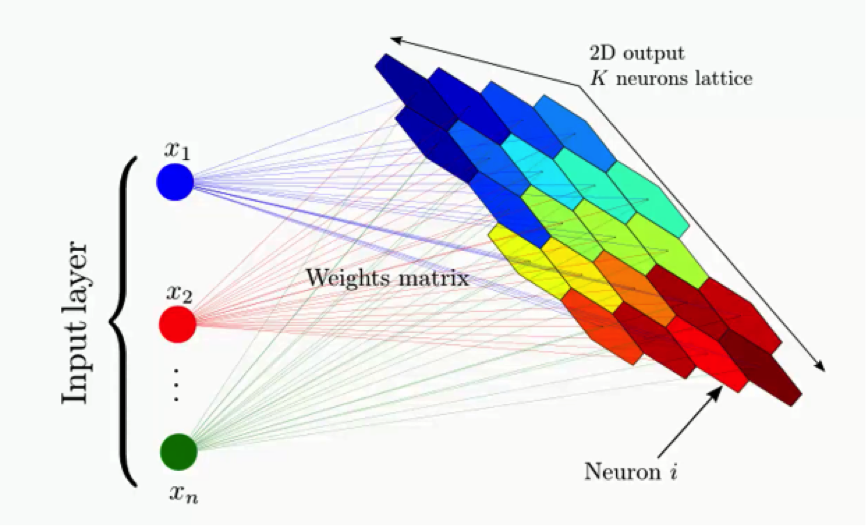
\includegraphics[width=0.8\textwidth]{imagenes/arquitectura_som.png}
\caption{Esquema de una red neuronal de Kohonen.}
\end{figure}
\section{Proceso de entrenamiento de un mapa autoorganizado.}
\textit{En la explicación de este algoritmo se asume que la capa de salida es una matriz bidimensional, como se ha comentado antes, esto no tiene que ocurrir aunque es lo más común.}\\

En primer lugar, se \textbf{inicializan} \textbf{los pesos} asociados a la capa de salida. Lo más habitual, es tomar dichos pesos de una distribución aleatoria.
Para un correcto funcionamiento dichos pesos deben estar normalizados entre 0 y 1. En nuestro caso, hemos tomado los pesos de una distribución aleatoria uniforme en el intervalo $[0, 1)$.\\

El proceso de entrenamiento que se presenta a continuación \textbf{se repite hasta que se alcanza el número de iteraciones máximo}, determinado por el parámetro $\lambda$. La variable $t$ representa cada una de las iteraciones.\\

Después, para cada una de las muestras, $X$, sacadas de la distribución de muestras, de forma aleatoria, se realizan los siguientes pasos: \\\\
1 - Se \textbf{calcula la distancia euclídea} entre la muestra $X$ y cada una de las neuronas de la capa de salida.\\
$$distancia(X) = || W - X ||$$\\
2 - Se \textbf{busca la neurona que ha obtenido una menor distancia}. Esta neurona es considerada la neurona ganadora o BMU \textit{(Best Matching Unit)}.\\
$$BMU_X = argmin_{W_{i, j}} \; distancia(X) = argmin_{W_{i, j}} || W - X ||$$\\
3 - Se realiza un \textbf{proceso de actualización de las matrices de pesos} en base a lo obtenido anteriormente, según la siguiente fórmula.\\
$$ W_{i, j}^{(t+1)} = W_{i, j}^{(t)} + \Delta {W_{i,j}} $$\\

La actualización depende tanto de la distancia de la muestra al vector de pesos como de otros dos parámetros: la tase de aprendizaje y una función de vecindario.\\

$$\Delta W_{i,j} = \eta(t)\delta_f(i,j)(X-W_{i,j})$$\\

La función $\delta_f(i,j)$ es la función de vecindario y, en nuestra se calcula conforme a la siguiente ecuación:\\

$$\delta_f(i,j) = e ^{-\frac{||BMU_X-(i,j)||^2}{2\sigma(t)^2}}. $$\\

Al tratar con una potencia con exponente negativo, un mayor valor absoluto de dicho exponente nos proporciona una valor de $\delta_f(i,j)$ menor. Por eso en el numerador se tiene en cuenta la distancia que hay entre la mejor neurona y la neurona actual. En el denominador se utiliza un parámetro de control $\sigma$que nos permite controlar la distancia que estamos considerando.\\\\

Normalmente, este parámetro, durante un primer número de iteraciones previamente proporcionado, de las consideradas en el proceso de entrenamiento, es inicializado a un valor alto $\sigma_0$ que decrece de manera exponencial conforme a otro parámetro de control $\tau$.


Una vez ha finalizado esa primera fase (han pasado $z$ iteraciones) se van refinando los resultados con un valor fijo mucho más bajo $\sigma_f$.\\


$$\sigma(t) = \left\{
\begin{array}{ll}
\sigma_0e^{-\frac{t}{\tau}} & si \;\;t < z\\
\sigma_f & si  \;\; t\geq z
\end{array}
\right.
$$\\

Para la tasa de aprendizaje se sigue una aproximación similar, la tasa de aprendizaje durante la primera fase está inicializada a un valor $\eta_0$ decreciendo conforme a una gaussiana y, una vez pasado un número de iteraciones, es fijado a un valor $\eta_f$. \\
$$\sigma(t) = \left\{
\begin{array}{ll}
\eta_0e^{-\frac{t}{\tau}} & si \;\;t < z\\
\eta_f & si  \;\; t\geq z
\end{array}
\right.$$\\

Así pues, este algoritmo acerca los pesos del vecindario de la BMU hacia la nueva muestra introducida para parecerse más a la misma. Esto lo hace teniendo en cuenta un vecindario alrededor de la BMU que decrece exponencialmente conforme pasa un número de iteraciones hasta quedarse fijo y una tasa de aprendizaje que también decrece exponencialmente hasta permanecer constante. \\Esto permite una primera fase de entrenamiento, con cambios más bruscos en la que se adaptan los valores completamente aleatorios para encontrar agrupamientos razonables. Conforme avanza dicha fase esos valores van decreciendo, hasta que quedan fijados permitiendo a la red neuronal refinar los agrupamientos obtenidos hasta ese momento.



\section{Implementación en CUDA.}
Antes de realizar la primera implementación en CUDA, analizamos las posibilidades de paralelización que nos aporta el algoritmo así como los accesos a memoria requeridos para utilizar las herramientas que cuda nos proporciona de la forma más eficiente posible.

\subsection{Grado de paralelismo.}
El algoritmo muestra una posibilidad de implementarlo de forma paralela innata. Cada vez que una muestra es tomada de la entrada todas las neuronas realizan las mismas operaciones con esa entrada. Por ello, la componente principal que va a determinar el grado de paralelismo que podríamos alcanzar como máximo viene dado por el número de neuronas que hay en la capa de salida. \\

Otra opción que sería interesante sería que el paralelismo dependiera del número de muestras procesadas, ya que, es mucho más frecuente a la hora de utilizar este tipo de modelos, especialmente al aplicarlos con el fin de realizar \textit{clustering} (agrupamiento de datos) o reducción de dimensionalidad que el número de muestras sea considerablemente superior al número de neuronas (grupos) que se desean obtener en la capa de salida. \\

Sin embargo, la dependencia de datos existente para actualizar la matriz de pesos en cada iteración genera una barrera de comunicación que evita que podamos plantear una solución eficiente del algoritmo estudiando basándonos en las muestras.

\subsection{Uso de memoria.}
En esta sección vamos a analizar las operaciones relacionadas con la memoria para poder tomar decisiones óptimas con respecto a ellas. \\

\underline{Transferencia de elementos del host al dispositivo.}\\
Cada vez que se invoca uno de los kernels utilizados para la resolución del algoritmo acabamos de obtener una nueva muestra dentro de una iteración. Para poder aprovechar la gran capacidad de paralelismo de la GPU es necesario que dichos elementos se encuentren la GPU, por ello, en esta implementación vamos a mover todo el conjunto de muestras al dispositivo antes de empezar a calcular el algoritmo, evitando así que se interrumpa la ejecución constante del dispositivo para recibir nuevas entradas a través del PCI Express 3.0.

Los parámetros de control, se mantendrán todos en la CPU y será necesario enviarlos para el kernel que se encargue de actualizar la matriz de pesos.\\

\underline{Uso de memoria compartida.}\\
El uso de la memoria compartida en una GPU es fundamental para poder obtener los mejores resultados. Esta memoria compartida es mucho más rápida que la memoria global del sistema ya que, en vez de hacer uso de la DRAM del dispositivo, los elementos de esta memoria se alojan en la caché L1 de la tarjeta permitiendo un acceso tanto para escritura como para lectura muy superior pero limitando a 48 KB el máximo de elementos que se pueden alojar por bloque de hebras en la misma.

En el algoritmo propuesto encontramos dos operaciones en las que podemos hacer uso de la memoria compartida.

\begin{itemize}
	\item A la hora de calcular la distancia euclídea, podemos guardar la muestra que estamos evaluando en memoria compartida, asegurándonos de que esta permanezca en la caché.
	\item A la hora de buscar el índice de la menor distancia, que se va a realizar mediante una técnica de reducción y que, por tanto, conlleva el uso de la memoria compartida para obtener buenos resultados.
\end{itemize}

\underline{Uso de la memoria del dispositivo.}\\
Todos los elementos generados en el dispositivo, se mantendrán en el mismo sin necesidad de ser transladados al host, salvo la matriz de pesos solución que una vez finalizada la ejecución del algoritmo se enviará al host. \\

\subsection{Kernels a desarrollar.}
Para obtener los mejores resultados hemos de intentar lanzar el menor número posible de kernels para evitar así los pequeños overheads que se dan para lanzar los mismos. Sin embargo, la naturaleza del algoritmo, que repite el proceso constantemente dificulta esta labor. \\

Antes de iniciar el bucle del algoritmo lanzaremos el primer kernel.\\

\underline{I - Inicialización aleatoria de pesos \textit{(cuda\_init\_weights)}.}\\

En el primer kernel vamos a inicializar aleatoriamente el array de pesos con valores sacados de una distribución uniforme de números reales en coma flotante entre 0 y 1. La generación de números aleatorios se realiza utilizando funciones que nos proporciona la librería Numba, cuya implementación se basa en el método de Box-Muller. \\\\

Este array de una única dimensión representa una estructura tridimensional basado en las filas de la matriz, las columnas de la matriz y la dimensión de los vectores de pesos.\\\\\\

En cada iteración del algoritmo se ejecuta lo siguiente:\\

\underline{II - Selección aleatoria de las muestras a usar \textit{(en CPU)}}\\
Puesto que el tamaño de muestras que se toma por iteración no tiende a ser muy grande, hemos optado por realizar esta opción en la CPU.\\

\underline{III - Cálculo de la distancia euclídea. \textit{(cuda\_euclidean\_distance)}} \\
Este kernel recibe una muestra y calcula la distancia euclídea de esa muestra con todos los elementos de la matriz de pesos. Para hacerlo de una manera más eficiente primero se introduce la muestra en memoria compartida y luego se calcula la distancia.

El array en el que se guardan las distancias resultantes permanece siempre en la memoria del dispositivo y es reutilizado de una iteración a otra. \\

\underline{IV - Encontrar menor distancia \textit{(amin() cuBLAS.)}} \\
En principio para solucionar este problema habíamos planteado una reducción. La reducción es una técnica común utilizada para computar eficientemente en una GPU una operación binaria que cumple la propiedad asociativa sobre todos los elementos de un array. El ejemplo más habitual de ello, es la suma. Puesto que la operación binaria mínimo cumple ese prerrequisito hemos planteado y desarrollado la solución con una reducción en la que tenemos en cuenta la dupla que conforman el valor y su índice en el array.

Este ha sido el objeto de más dificultad de esta implementación y, aunque hemos conseguido una implementación considerablemente eficiente especialmente ante una implementación secuencial, hemos considerarlo sustituirlo por el método amin() de la librería altamente optimizada de cuBLAS que calculaba los resultados entre 2 y 4 veces más rápido (dependiendo del tamaño de la entrada), que nuestra implementación.\\

\underline{ V - Actualización de la matriz de pesos \textit{(cuda\_bmu\_update)}} \\
Este kernel recibe los parámetros de control y aplica la actualización de los pesos conforme a lo descrito en la fase de actualización del algoritmo explicado en la sección anterior (3.3).
